\section{Global System View}

The proposed system aims to aid the study of the dynamics associated with the wave breaking process.  The system consists of a base station, which is composed of a computer with the necessary software and hardware components to communicate with the spheres, which comprise the rest of the system.  The system must be able to handle at least five spheres at once with a single base station.

The spheres are meant to emulate fluid particles in movement as they are carried by the waves.  For this reason, the spheres should be as small as possible so that they could better emulate the particles of a fluid.  Previous work has been done with spheres of 7.5 cm in diameter \cite{Canals2012}, however these capsules lacked some of the capabilities that are proposed in this work.  One of the goals of this work is to attempt to add the extra functionality while keeping the current sphere dimensions.

The spheres should be transparent with the printed circuit boards containing the necessary circuitry aligned as much as possible with a single axis to ensure an axisymmetric design.  Figure~\ref{fig:sphereMockup} shows a very rough model of what the spheres should look like.  Note that this model does not aim to accurately depict the final product, but rather to give the reader a visual idea of the devices this report has tried and continues to describe.  

\begin{figure}[H]
	\centering
	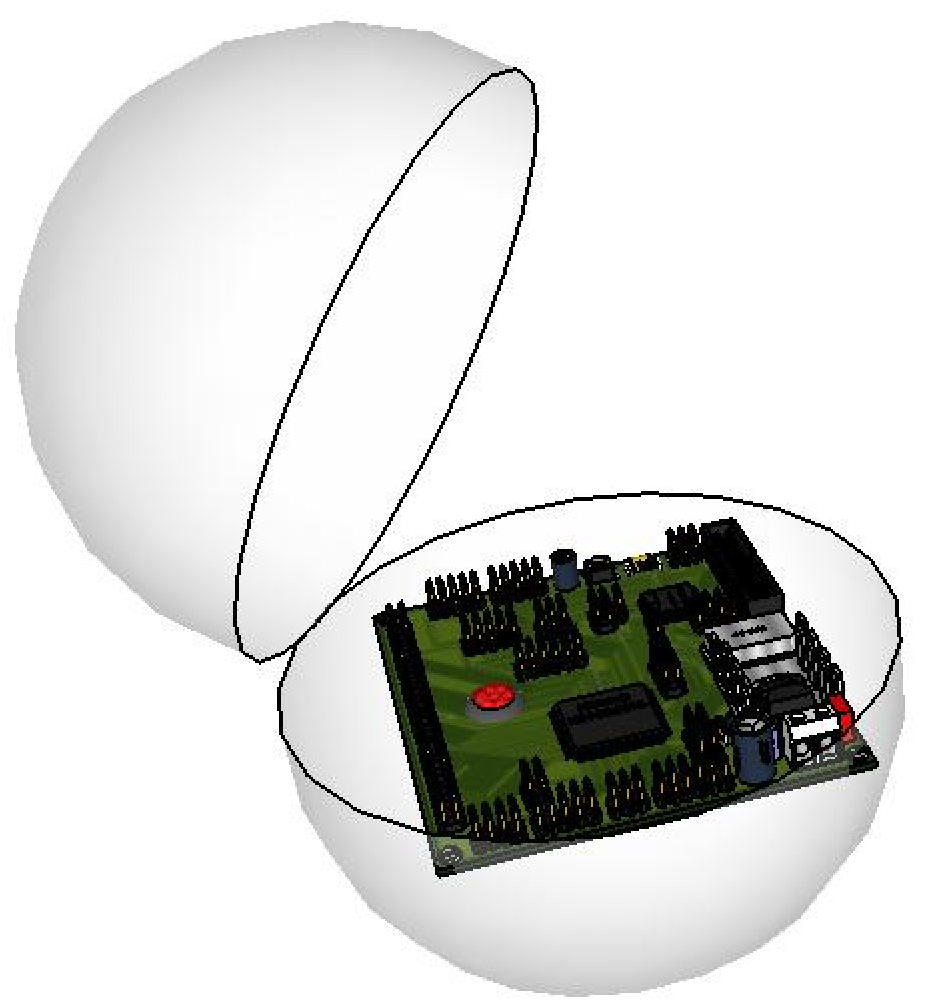
\includegraphics[scale=0.6]{img/Sphere_001.png}
	\caption{A rough model of the spheres. \label{fig:sphereMockup}}
\end{figure}

Each sphere must perform a series of tasks in a specific order during an experiment.  First, the sphere will be activated wirelessly by the base station and will be signaled to start collecting data.  The sphere will then be thrown into the waves, where it will continue to collect and save data continuously for at least 30 seconds. Once the sampling is completed, the sphere will attempt to signal its location, as determined by the GPS module inside, to the base station.  At the same time, if the light sensors indicate that the experiment is being conducted at night, the indicator lights must start flashing in order to aid the researchers in the search for the sphere.  Figure~\ref{fig:GSV} shows how the experiments will be conducted by the researchers.  They will have a laptop on a jet ski with the necessary hardware and software and at least one sphere to throw into the water.  The spheres and the computer communicate between each other to accomplish the goals of the experiments.

\begin{figure}[H]
	\centering
	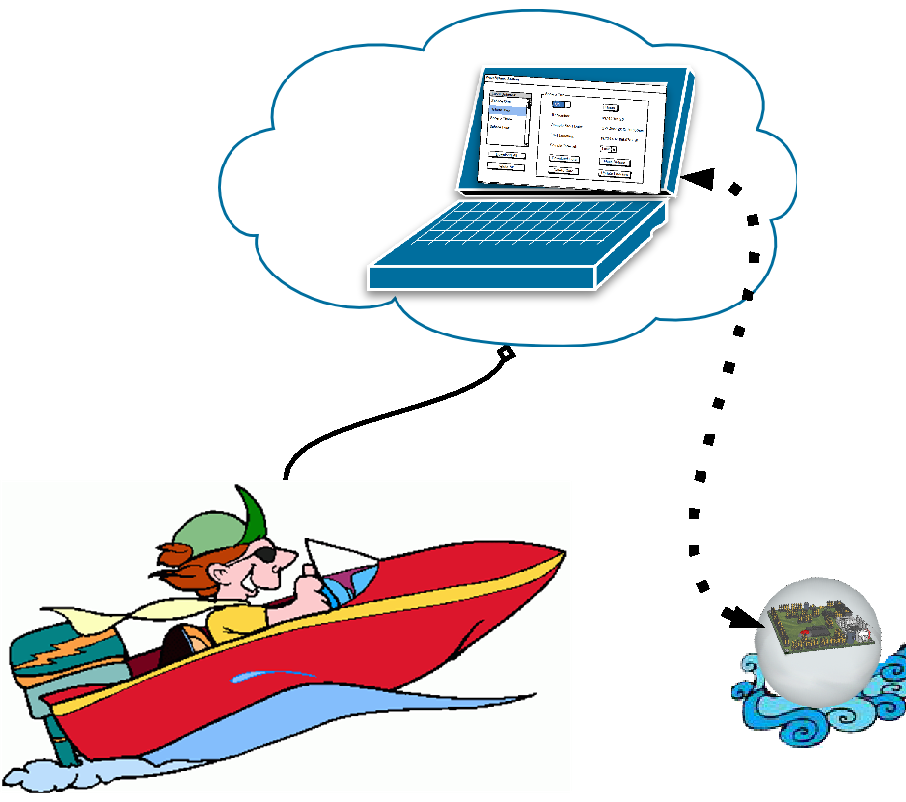
\includegraphics[scale=0.6]{img/GSV1}
	\caption{A rough model of the interaction between the system. \label{fig:GSV}}
\end{figure}

Once the sphere has been recovered, it needs be either reset for another experiment, set in data transfer mode or deactivated.  The base station will allow the user to select one of these options.  If the user resets the sphere for another experiment, then the previously described process is repeated without deleting the data of the previous experiment.  After this point, if the sphere does not have enough memory to perform another experiment, then the base station should alert the user and at the same time an LED will light up in a particular manner to call attention to this situation. If the user chooses to deactivate the sphere, the data must persist in the mass storage until it is retrieved. If the user instead selects the option to transfer the data, then the sphere will enter the data transfer mode and will indicate the user that the process has begun by flashing a blue LED.  At the same time, the software at the base station will indicate to the user that the data transfer process is underway.  The base station must acquire the data in each sphere and create a separate file to save the data acquired for each experiment.  After this, the user should be asked if they wish to delete the data on the mass storage in the sphere.  If they select this option, then all the data from previous experiments will be deleted.  After the data transfer has concluded, the sphere will deactivate itself and return to the original state described earlier.





